\chapter{Datos y Cohorte}
\label{chapter:datos_cohorte}

Los datos utilizados en este trabajo provienen de la \textit{Red Latinoamericana de Investigación en Neurodegeneración} (RedLaT), una iniciativa colaborativa que integra información clínica y de neuroimagen recolectada en múltiples centros de América Latina. El objetivo general del proyecto es mejorar la caracterización de la demencia en poblaciones históricamente subrepresentadas, incorporando datos multimodales que permitan estudiar procesos de envejecimiento cerebral y neurodegeneración en un contexto regional diverso.

A diferencia de muchas bases de datos empleadas en estudios de conectividad cerebral, construidas mayormente a partir de cohortes europeas o norteamericanas, RedLaT representa una población latinoamericana con una marcada heterogeneidad genética, cultural y socioeconómica. Esta diversidad resulta particularmente relevante para evaluar la generalización de modelos desarrollados en otros contextos y para explorar posibles moduladores regionales de la variabilidad interindividual asociada al envejecimiento cerebral y a patologías neurodegenerativas.

\section{Fuentes de datos}
\label{sec:fuentes_datos}

En este trabajo se integran tres fuentes principales de información:
\begin{itemize}
    \item \textbf{Conectividad funcional (FC):} matrices de $116 \times 116$ estimadas a partir de fMRI en estado de reposo (véase Sección~\ref{sec:conectividad_funcional} del Capítulo~\ref{chapter:marco_teorico}), que cuantifican la dependencia temporal entre regiones cerebrales definidas por el atlas AAL.
    \item \textbf{Metadatos clínicos y demográficos:} edad, sexo, diagnóstico clínico (controles sanos, CN; enfermedad de Alzheimer, AD; demencia frontotemporal, FTD), años de educación formal, sitio de adquisición y marca del escáner de resonancia magnética.
    \item \textbf{Medidas estructurales T1w:} 116 valores regionales de volumen de materia gris derivados de morfometría basada en vóxeles (VBM), como se describe en la Sección~\ref{sec:mri} del Capítulo~\ref{chapter:marco_teorico}.
\end{itemize}

Tanto las matrices de conectividad funcional como las medidas estructurales se encuentran definidas sobre el mismo atlas AAL de 116 regiones (véase Sección~\ref{sec:conectividad_funcional} del Capítulo~\ref{chapter:marco_teorico}), lo que permite establecer una correspondencia directa entre modalidades a nivel regional.


\section{Integración de fuentes y construcción de la cohorte}
\label{sec:construccion_cohorte}

Las distintas fuentes de datos presentan identificadores heterogéneos. Para unificar criterios, se aplicó un procedimiento de limpieza y normalización orientado a recuperar un identificador unívoco (\texttt{record\_id}) a partir de nombres de archivo y campos textuales. A partir de esta etapa se obtuvo un conjunto inicial de sujetos con datos funcionales disponibles, que luego se cruzó con los metadatos clínicos y con las medidas estructurales T1w.

La Figura~\ref{fig:cohort_flow} resume esquemáticamente el flujo de integración y filtrado. Dado que la edad constituye la variable objetivo principal de este trabajo, se excluyeron aquellos sujetos sin edad registrada. El resultado es una cohorte final única, compuesta por sujetos con información funcional, estructural y clínica completa.

\begin{figure}[H]
\centering
\resizebox{\textwidth}{!}{%
\begin{tikzpicture}[
  box/.style={
    draw,
    rounded corners,
    align=center,
    text width=5cm,
    inner sep=7pt
  },
  arr/.style={-Latex, thick},
  font=\small
]
\node[box] (fc) {Matrices FC\\\textbf{N=1365}};
\node[box, right=18mm of fc] (meta) {Metadatos clínicos\\CN/AD/FTD, edad\\\textbf{N=1327}};
\node[box, below=16mm of meta] (t1) {Medidas T1w\\\textbf{N=2748}};
\node[box, left=18mm of t1] (final) {Cohorte final\\FC $\cap$ Meta $\cap$ T1w\\\textbf{N=1245}};

\draw[arr] (fc) -- node[midway, above]{\scriptsize (1)} (meta);
\draw[arr] (meta) -- node[midway, right]{\scriptsize (2)} (t1);
\draw[arr] (t1) -- node[midway, below]{\scriptsize (3)} (final);
\end{tikzpicture}}
\caption{
Proceso de integración de datos.
(1) Metadatos clínicos filtrados por diagnóstico (CN, AD, FTD) y disponibilidad de edad.
(2) Intersección con medidas estructurales T1w (un sujeto por \texttt{record\_id}, duplicados promediados).
(3) Intersección con matrices FC disponibles. Cohorte final: N=1245.
}
\label{fig:cohort_flow}
\end{figure}


\section{Descripción demográfica y clínica}
\label{sec:descripcion_cohorte}

La Tabla~\ref{tab:diag_dist} resume la composición diagnóstica de la cohorte final, que comprende tres grupos: controles sanos (CN), pacientes con enfermedad de Alzheimer (AD) y pacientes con demencia frontotemporal (FTD). La distribución por sexo se reporta en la Tabla~\ref{tab:sex_dist}.

\begin{table}[H]
\centering
\begin{tabular}{lrr}
\toprule
 & Conteo & Porcentaje \\
\midrule
CN & 526 & 42.2 \\
AD & 422 & 33.9 \\
FTD & 297 & 23.9 \\
\bottomrule
\end{tabular}
\caption{Distribución diagnóstica en la cohorte final (N=1245).}
\label{tab:diag_dist}
\end{table}


\begin{table}[H]
\centering
\begin{tabular}{lrr}
\toprule
 & Conteo & Porcentaje \\
\midrule
Male & 767 & 61.6 \\
Female & 478 & 38.4 \\
\bottomrule
\end{tabular}
\caption{Distribución por sexo en la cohorte final (N=1245).}
\label{tab:sex_dist}
\end{table}


La Tabla~\ref{tab:age_summary} resume la distribución de la edad en la cohorte final mediante estadísticas descriptivas de tendencia central y dispersión.

\begin{table}[H]
\centering
\begin{tabular}{rrrrrl}
\toprule
N & Media & DE & Mediana & IQR & Min--Max \\
\midrule
1245 & 66.1 & 10.2 & 67.0 & 14.0 & 18.0--98.0 \\
\bottomrule
\end{tabular}
\caption{Resumen descriptivo de la edad en la cohorte final.}
\label{tab:age_summary}
\end{table}



\section{Distribución etaria y comparación por diagnóstico}
\label{sec:distribucion_etaria}

La Figura~\ref{fig:age_hist} muestra la distribución de edades en la cohorte final. 
Se observa un rango amplio (18--98 años), con una mayor concentración de sujetos en edades medias y avanzadas (mediana = 67 años), sin la presencia de discontinuidades o acumulaciones atípicas evidentes.

En complemento, la Figura~\ref{fig:age_by_diag_box} compara la distribución de la edad entre diagnósticos clínicos. 
Si bien se observan diferencias en la mediana y en la dispersión entre grupos, los rangos etarios presentan una superposición considerable, lo que indica que la edad por sí sola no discrimina de manera clara entre los diagnósticos considerados. Este solapamiento es relevante para el modelado: un modelo de predicción de edad no puede apoyarse únicamente en la etiqueta diagnóstica como proxy de la edad.

\begin{figure}[H]
    \centering
    \begin{subfigure}[t]{0.48\textwidth}
        \centering
        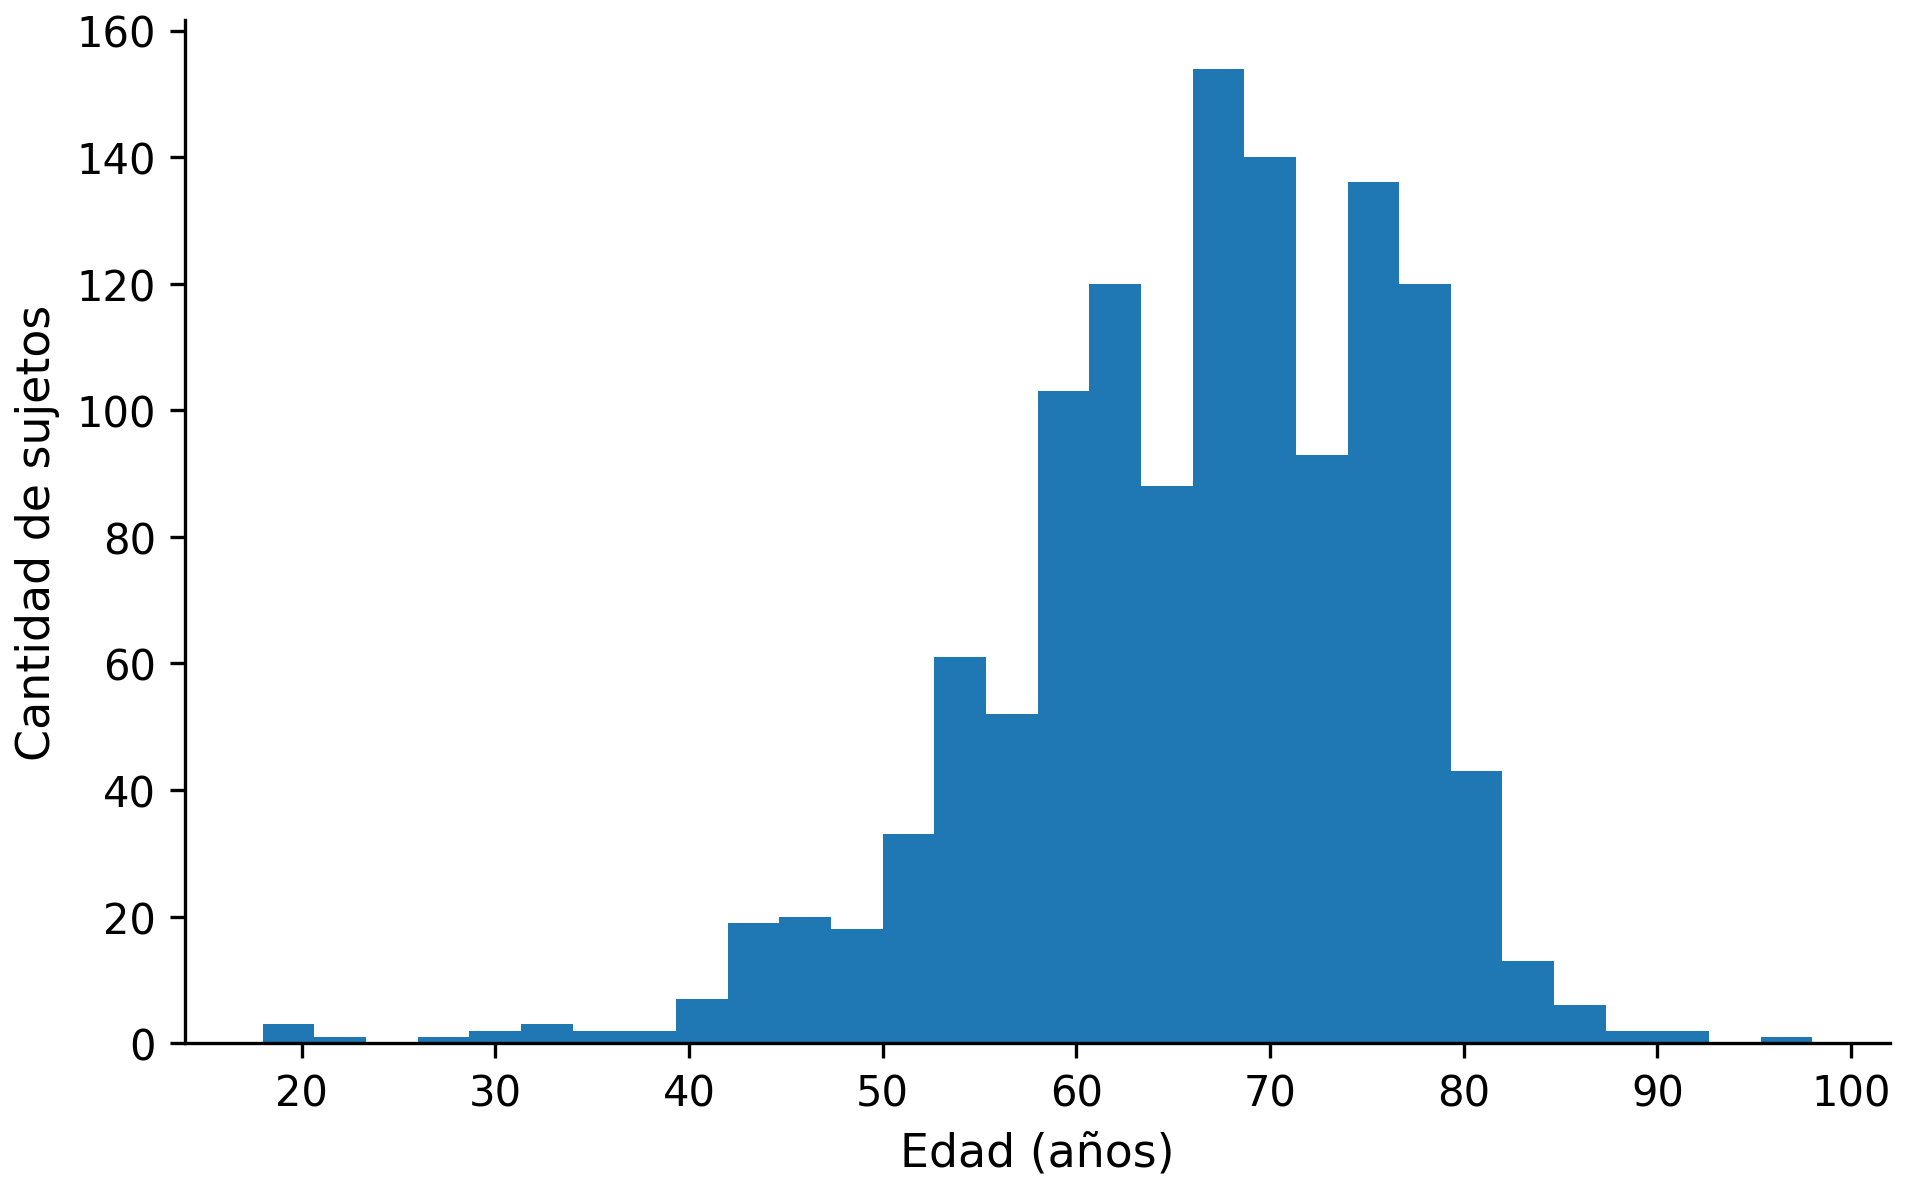
\includegraphics[width=\textwidth]{05_datos_cohorte/images/age_hist.png}
        \caption{Distribución de edades en la cohorte final.}
        \label{fig:age_hist}
    \end{subfigure}
    \hfill
    \begin{subfigure}[t]{0.48\textwidth}
        \centering
        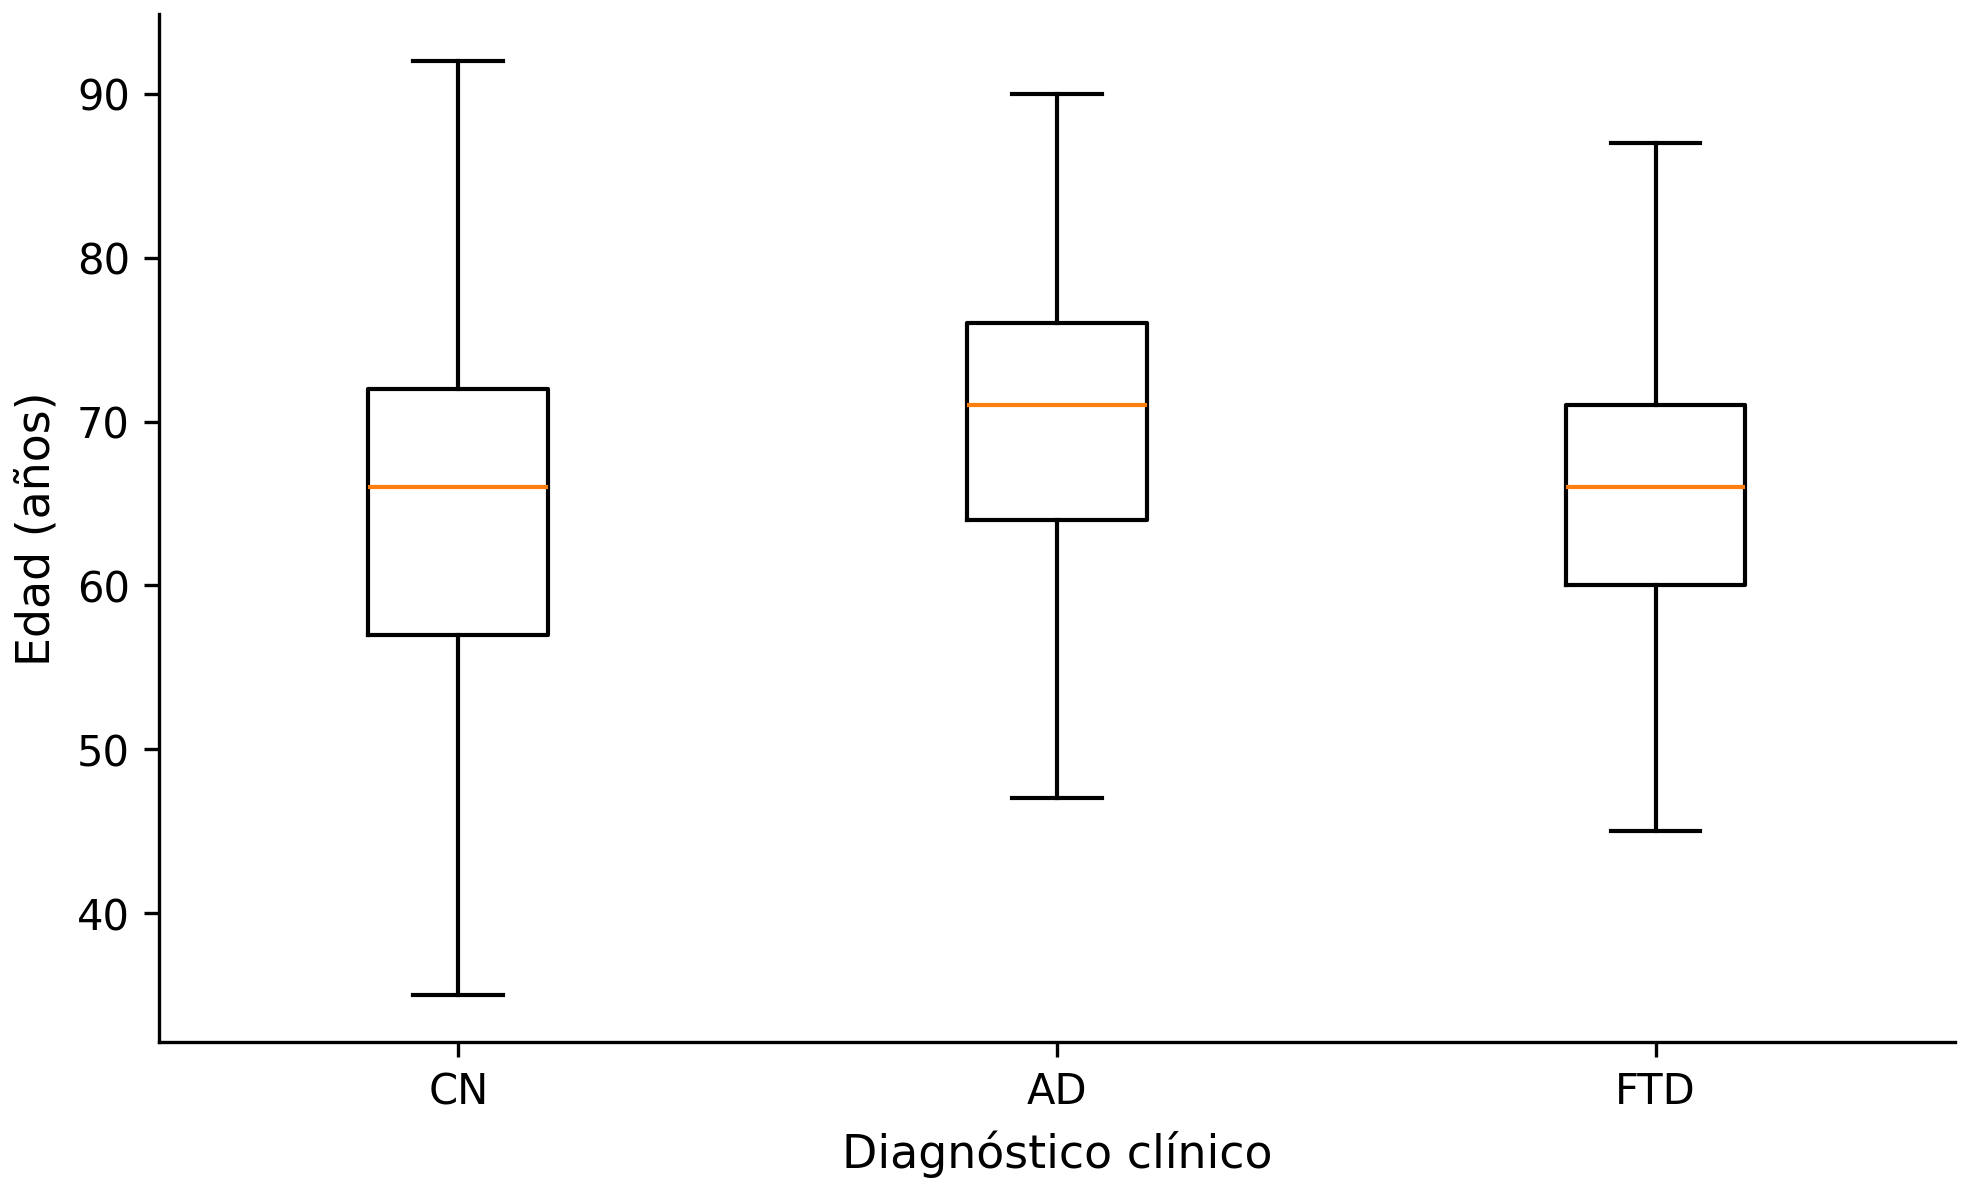
\includegraphics[width=\textwidth]{05_datos_cohorte/images/age_by_diag_box.png}
        \caption{Distribución de la edad por diagnóstico clínico.}
        \label{fig:age_by_diag_box}
    \end{subfigure}
    \caption{Caracterización de la distribución etaria global y estratificada por diagnóstico.}
    \label{fig:age_combined}
\end{figure}


\section{Balance por sexo dentro de cada diagnóstico}
\label{sec:balance_sexo}

Más allá de la distribución global por sexo, es útil evaluar el balance \emph{dentro} de cada diagnóstico. La Figura~\ref{fig:sex_by_diag} muestra la composición porcentual por sexo estratificada por diagnóstico. Se observa un predominio masculino en todos los grupos, más acentuado en CN y AD ($\sim$66\% masculino) y más equilibrado en FTD ($\sim$51\% masculino). Estos desbalances son potencialmente relevantes como factores de confusión y deben tenerse en cuenta al interpretar los resultados del modelo.

\begin{figure}[H]
    \centering
    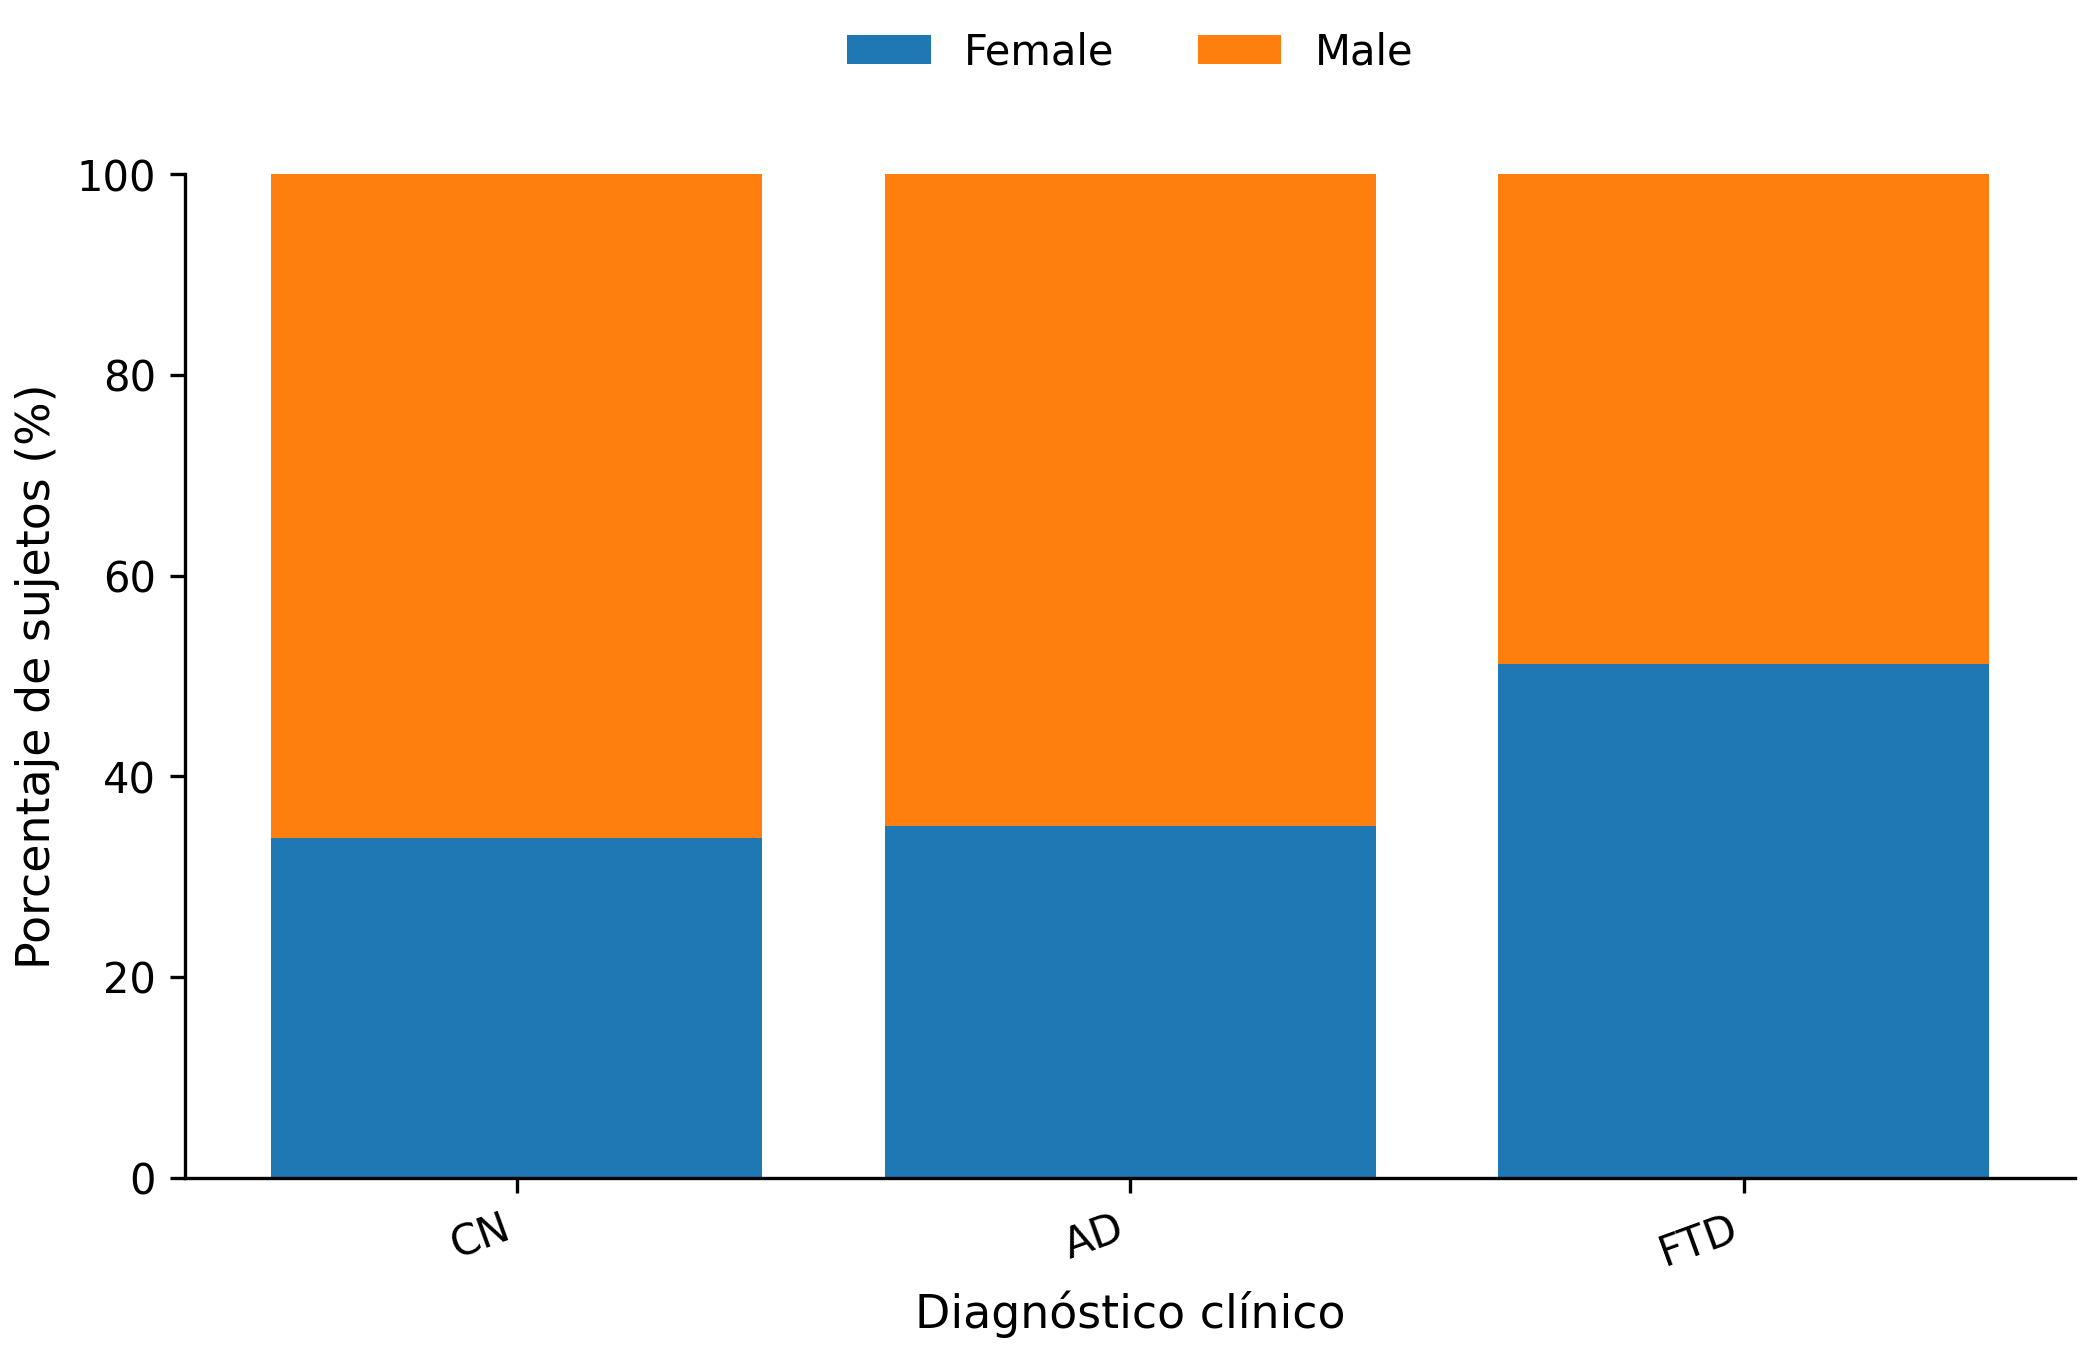
\includegraphics[width=0.82\textwidth]{05_datos_cohorte/images/sex_by_diag_stacked.png}
    \caption{Distribución porcentual por sexo estratificada por diagnóstico clínico.}
    \label{fig:sex_by_diag}
\end{figure}


\section{Variables demográficas adicionales}
\label{sec:demo_adicionales}

Además de la edad, el sexo y el diagnóstico clínico, el archivo de metadatos de RedLaT contiene variables demográficas que no se utilizan como entrada del modelo principal pero resultan relevantes para analizar factores de confusión y moduladores de la predicción de edad cerebral. La Tabla~\ref{tab:demo_availability} resume la disponibilidad de estas variables dentro de la cohorte final.

\begin{table}[H]
\centering
\caption{Disponibilidad de variables demográficas adicionales en la cohorte final ($N = 1245$). Las variables no están completas para todos los sujetos, lo que debe considerarse al interpretar los análisis que las utilizan.}
\label{tab:demo_availability}
\begin{tabular}{llrr}
\toprule
\textbf{Variable} & \textbf{Descripción} & \textbf{Disponibles} & \textbf{\%} \\
\midrule
\texttt{cog\_ed}           & Años de educación formal            & 933  & 74,9\% \\
\texttt{site}              & Sitio de adquisición (centro)       & 941  & 75,6\% \\
\texttt{mri\_scanner\_brand} & Marca del escáner MRI               & 921  & 74,0\% \\
\texttt{mmse\_total}        & Puntuación MMSE                     & 923  & 74,1\% \\
\bottomrule
\end{tabular}
\end{table}

\paragraph{Años de educación (\texttt{cog\_ed}).} Esta variable registra los años de educación formal completados por cada sujeto, y constituye el indicador de nivel socioeconómico más directamente disponible en la cohorte. Los valores oscilan entre 0 y 25 años. Estratificado por diagnóstico, los controles sanos presentan un nivel educativo más alto (media $\approx 16{,}2$ años) que los pacientes con AD ($\approx 12{,}9$ años) y FTD ($\approx 14{,}4$ años). La educación es un factor particularmente relevante en el contexto latinoamericano, donde la variabilidad en el acceso a la educación formal es considerable y puede modular tanto la expresión clínica de la neurodegeneración como el acceso al diagnóstico.

\paragraph{Sitio de adquisición (\texttt{site}).} La cohorte integra datos de múltiples centros de investigación distribuidos en varios países latinoamericanos. Los sitios con mayor representación son Miller ($n = 400$), Matallana ($n = 135$), Slachevsky ($n = 93$), Takada ($n = 89$), Lopera ($n = 88$) y Behrens ($n = 60$). Cada centro utiliza protocolos de adquisición potencialmente distintos, lo que introduce una fuente de variabilidad técnica que puede actuar como factor de confusión en los modelos de predicción.

\paragraph{Marca del escáner MRI (\texttt{mri\_scanner\_brand}).} Los escáneres empleados corresponden a tres fabricantes principales: Siemens ($n = 581$, 63\%), GE ($n = 289$, 31\%) y Philips ($n = 47$, 5\%). Las diferencias en hardware, secuencias de pulso y algoritmos de reconstrucción entre fabricantes pueden producir variaciones sistemáticas en las imágenes, un fenómeno conocido como \textit{scanner bias}. Este sesgo técnico puede manifestarse como diferencias artificiales en las medidas derivadas de la neuroimagen, incluso cuando los cerebros subyacentes son comparables.

La puntuación MMSE (\textit{Mini-Mental State Examination}) se incluye en la tabla por completitud, pero no se utiliza como feature en el pipeline de predicción de edad, ya que es una medida de estado cognitivo que está directamente correlacionada con el diagnóstico clínico y no constituye un predictor independiente del envejecimiento cerebral normal.

Dado que estas variables no están disponibles para la totalidad de la cohorte, los análisis que las utilizan (Capítulo~\ref{chapter:resultados_discusion}) operan sobre subconjuntos de menor tamaño que los $N = 1245$ sujetos del pipeline principal.


\section{Análisis exploratorio}
\label{sec:analisis_exploratorio}

Como control descriptivo previo al modelado, se exploraron relaciones entre la edad y medidas globales derivadas de las dos modalidades de neuroimagen. Para cuantificar estas relaciones se utilizan coeficientes de correlación, que se describen a continuación antes de presentar los resultados.

El \textbf{coeficiente de correlación de Pearson} ($r$) mide la fuerza de la relación lineal entre dos variables. Su valor va de $-1$ a $+1$: un valor de $r = +1$ significa que cuando una variable sube, la otra siempre sube proporcionalmente; $r = -1$ significa que cuando una sube, la otra siempre baja; y $r = 0$ indica que no hay ningún patrón lineal entre ambas. A modo de referencia, valores de $|r|$ entre 0{,}1 y 0{,}3 indican una relación débil, entre 0{,}3 y 0{,}5 moderada, y por encima de 0{,}5 fuerte.

El \textbf{coeficiente de Spearman} ($\rho$) responde a la misma pregunta que el de Pearson, pero no exige que la relación sea una línea recta. En vez de operar sobre los valores numéricos directos, utiliza las posiciones ordenadas (rangos) de los datos, lo que lo hace más resistente a valores extremos y capaz de detectar relaciones curvas o no lineales. Su interpretación es análoga: $\rho = +1$ indica una relación monótona creciente perfecta, $\rho = -1$ decreciente perfecta, y $\rho = 0$ ausencia de tendencia.

El \textbf{valor $p$} acompaña a ambos coeficientes e indica la probabilidad de que la relación observada se deba al azar. Un $p$ bajo significa que es muy improbable que el patrón sea una coincidencia. Por convención, si $p < 0{,}05$ se dice que el resultado es \textit{estadísticamente significativo}: podemos confiar en que la relación detectada es real y no un artefacto del muestreo.

Estas métricas se utilizan a lo largo de este capítulo y del Capítulo~\ref{chapter:resultados_discusion} para evaluar asociaciones entre variables.

\subsection{Edad y volumen de materia gris}

La Figura~\ref{fig:corr_age_gm} muestra la relación entre la edad y el volumen promedio de materia gris por sujeto. Para cada persona, este valor se calcula promediando los 116 volúmenes regionales de materia gris (uno por cada región del atlas AAL), obteniendo un único número que resume la cantidad global de materia gris en su cerebro.

Se observa una correlación negativa moderada (Pearson $r = -0{,}30$, $p < 0{,}001$), lo que significa que las personas de mayor edad tienden a tener menos materia gris. El coeficiente de Spearman ($\rho = -0{,}24$) confirma esta tendencia. Este resultado es consistente con la evidencia de que el volumen de materia gris disminuye progresivamente con la edad (véase Sección~\ref{sec:bases_neuro} del Capítulo~\ref{chapter:marco_teorico}). La dispersión considerable indica que, si bien la tendencia global es clara, existe una marcada variabilidad entre individuos: dos personas de la misma edad pueden tener cantidades de materia gris bastante diferentes.

\begin{figure}[H]
    \centering
    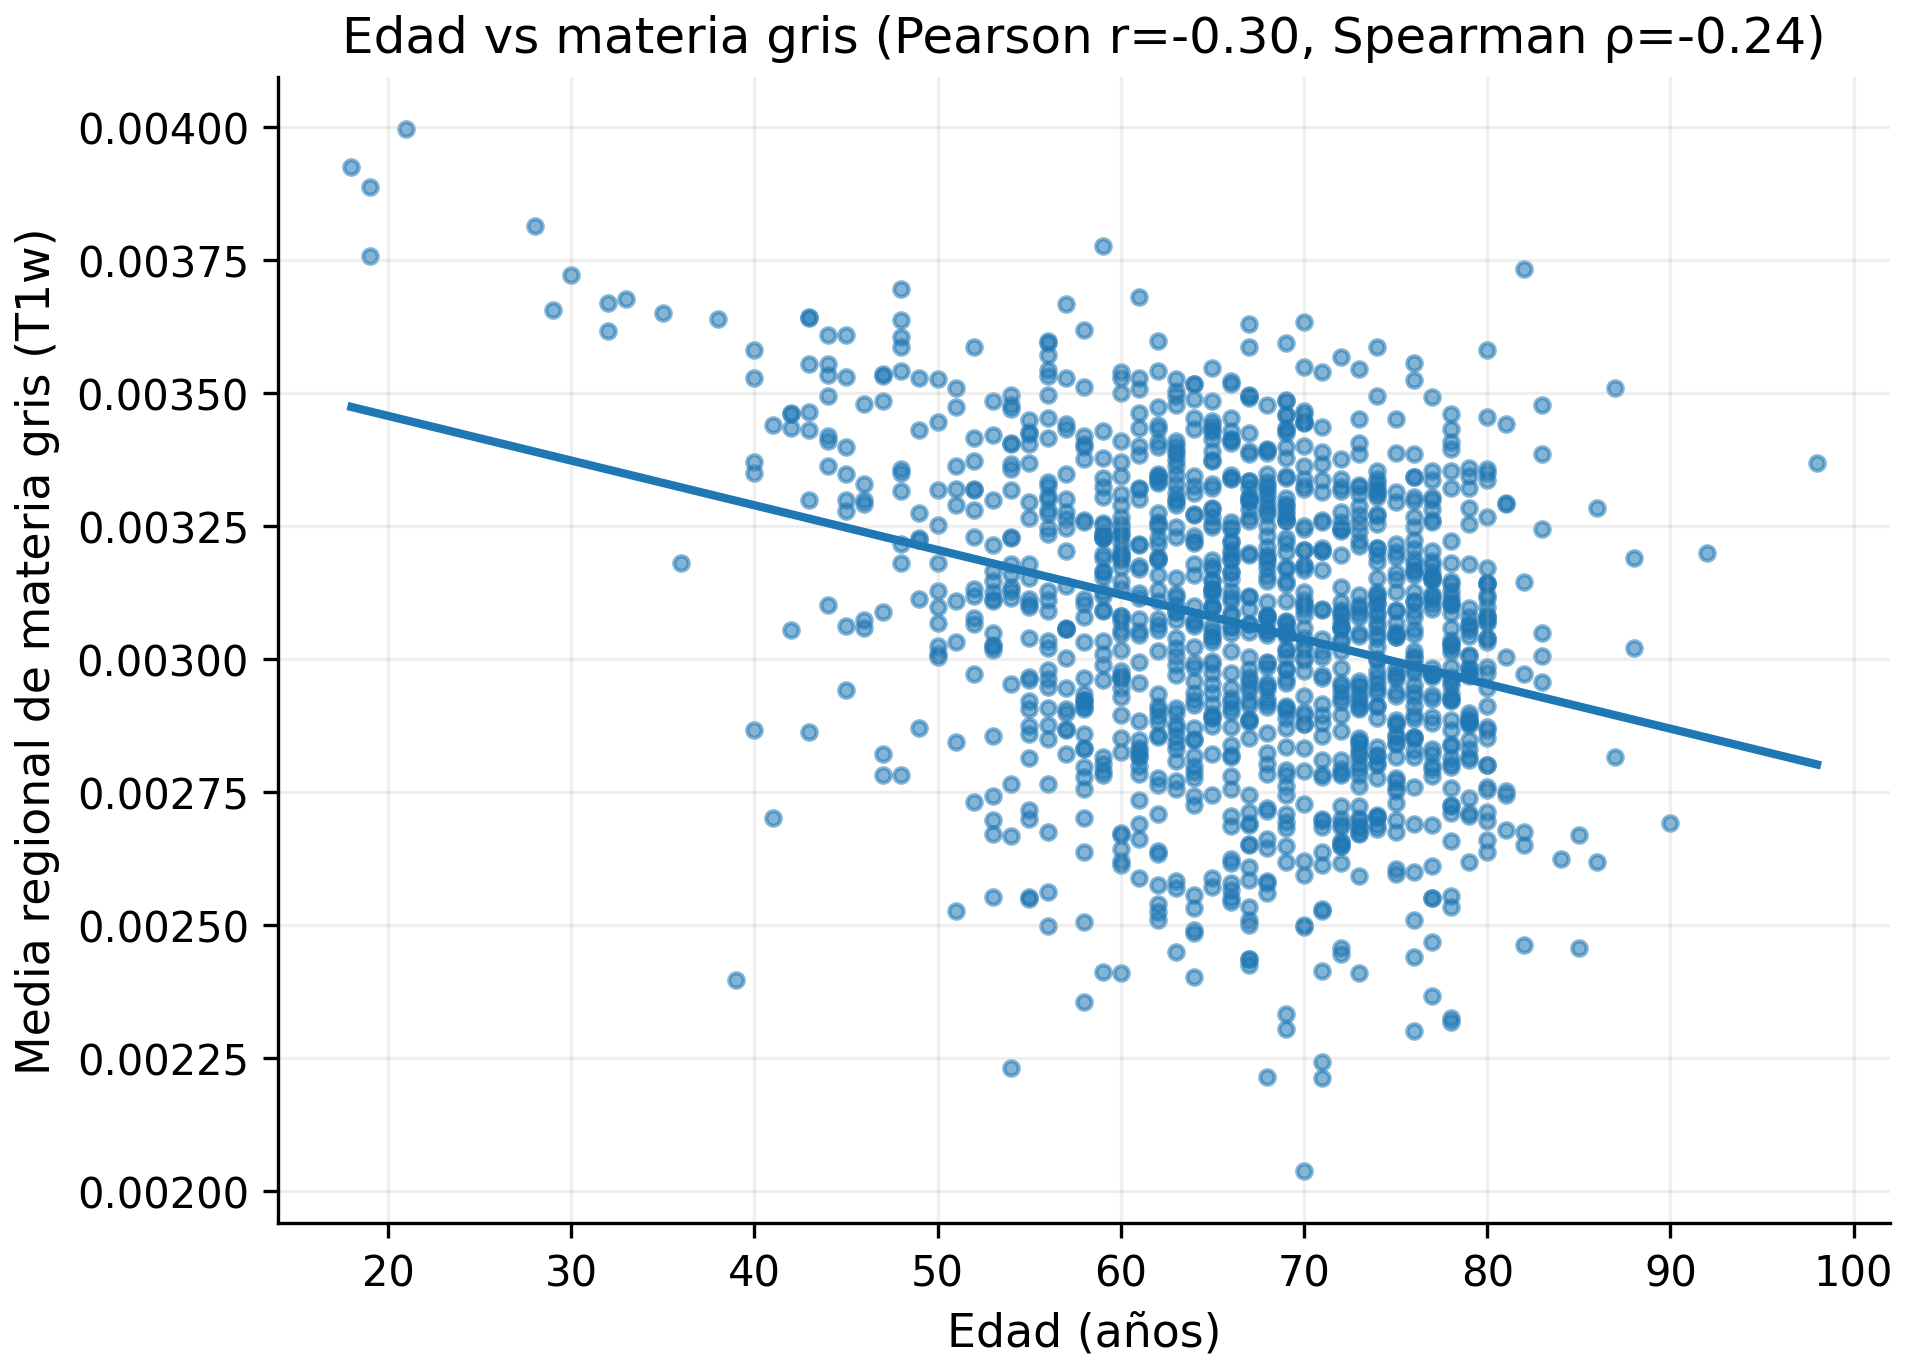
\includegraphics[width=0.78\textwidth]{05_datos_cohorte/images/corr_age_gmmean.png}
    \caption{Edad versus promedio regional de materia gris (T1w). Cada punto corresponde a un sujeto y la recta indica la tendencia lineal.}
    \label{fig:corr_age_gm}
\end{figure}

\subsection{Edad y conectividad funcional global}

De manera complementaria, la Figura~\ref{fig:corr_age_fc} evalúa una medida global simplificada de conectividad funcional: para cada sujeto se calcula el promedio de las correlaciones absolutas entre todos los pares de regiones cerebrales de su matriz FC, obteniendo un único número que resume la fuerza general de la conectividad. En este caso, la correlación con la edad es prácticamente nula (Pearson $r \approx 0{,}00$, Spearman $\rho \approx -0{,}01$), lo que indica que esta medida global no captura los efectos del envejecimiento.

Este resultado no implica que la conectividad funcional no contenga información sobre la edad, sino que dicha información probablemente reside en patrones específicos de conectividad entre regiones y no en una medida agregada global. Esta observación justifica el uso de métodos de reducción de dimensionalidad no lineales (como el $\beta$-VAE descrito en la Sección~\ref{sec:beta_vae_theory} del Capítulo~\ref{chapter:marco_teorico}) que pueden capturar relaciones más complejas entre las 6670 conexiones individuales.

\begin{figure}[H]
    \centering
    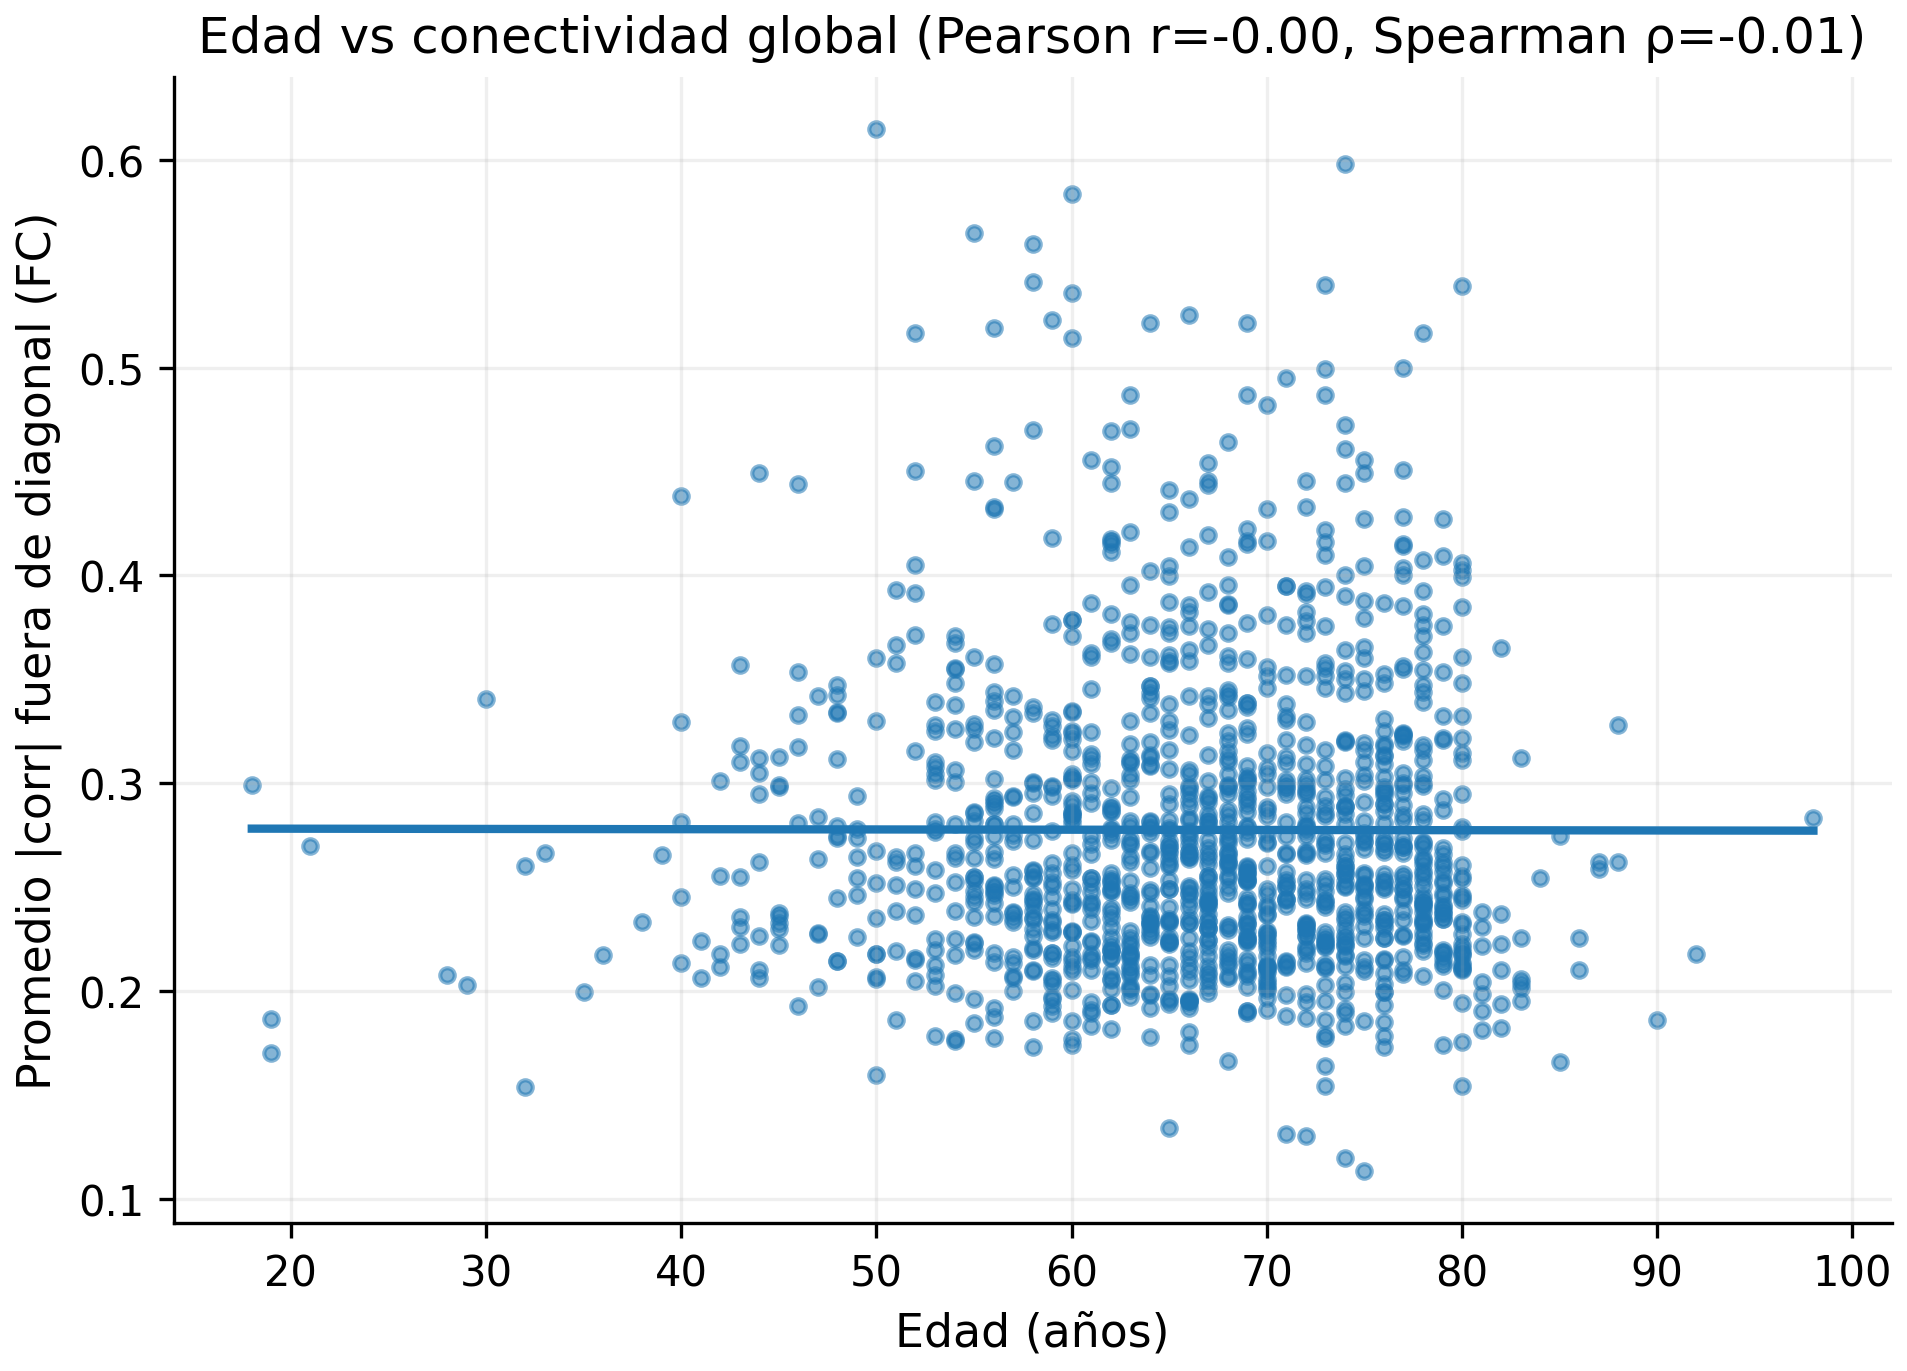
\includegraphics[width=0.78\textwidth]{05_datos_cohorte/images/corr_age_fcmean.png}
    \caption{Edad versus conectividad funcional global (promedio de $|corr|$ fuera de la diagonal). La ausencia de correlación sugiere que los efectos del envejecimiento en FC no se reflejan en una métrica agregada.}
    \label{fig:corr_age_fc}
\end{figure}


\section{Consideraciones poblacionales}
\label{sec:consideraciones_poblacionales}

El uso de una cohorte latinoamericana permite estudiar el envejecimiento cerebral y la neurodegeneración en un contexto poblacional distinto al de cohortes de referencia como ADNI o UK Biobank. Factores asociados a diversidad genética, condiciones de vida, acceso a sistemas de salud y contexto sociocultural podrían contribuir a la variabilidad interindividual observada en medidas funcionales y estructurales. La heterogeneidad en los niveles educativos y en los protocolos de adquisición entre centros, descritas en la Sección~\ref{sec:demo_adicionales}, añade una fuente de variabilidad propia de cohortes multicéntricas latinoamericanas, cuyo impacto sobre la predicción de edad se cuantifica en el Capítulo~\ref{chapter:resultados_discusion}. En conjunto, los análisis presentados en este capítulo describen las principales características de la cohorte de estudio y proporcionan el contexto necesario para la metodología empleada en el Capítulo~\ref{chapter:metodologia_pipeline}.
